\documentclass[letterpaper,11pt]{article}

% Soporte para los acentos.
\usepackage[utf8]{inputenc}
\usepackage[T1]{fontenc}
% Idioma español.
\usepackage[spanish,mexico, es-tabla]{babel}
% Soporte de símbolos adicionales (matemáticas)
\usepackage{multirow}
\usepackage{amsmath}
\usepackage{amssymb}
\usepackage{amsthm}
\usepackage{amsfonts}
\usepackage{mathtools}
\usepackage{latexsym}
\usepackage{enumerate}
\usepackage{ragged2e}
\usepackage{listings}
\usepackage{xcolor}
\usepackage{graphicx}
\usepackage{hyperref}
\usepackage[linguistics]{forest}
% Modificamos los márgenes del documento.                                       %
\usepackage[lmargin=2cm,rmargin=2cm,top=2cm,bottom=2cm]{geometry}

\definecolor{codegreen}{rgb}{0,0.6,0}
\definecolor{codegray}{rgb}{0.5,0.5,0.5}
\definecolor{codepurple}{rgb}{0.58,0,0.82}
\definecolor{backcolour}{rgb}{0.95,0.95,0.92}

\lstdefinestyle{mystyle}{
    backgroundcolor=\color{backcolour},   
    commentstyle=\color{codegreen},
    keywordstyle=\color{magenta},
    numberstyle=\tiny\color{codegray},
    stringstyle=\color{codepurple},
    basicstyle=\ttfamily\footnotesize,
    breakatwhitespace=false,         
    breaklines=true,                 
    captionpos=b,                    
    keepspaces=true,                 
    numbers=left,                    
    numbersep=5pt,                  
    showspaces=false,                
    showstringspaces=false,
    showtabs=false,                  
    tabsize=2
}

\lstset{style=mystyle}

\title{Facultad de Ciencias, UNAM \\ Análisis de Algoritmos \\ Tarea 1}
\author{Rubí Rojas Tania Michelle}
\date{09 de octubre de 2020}

\begin{document}
\maketitle

\begin{enumerate}
    % Ejercicio 1.
    \item ¿Cuántas comparaciones son necesarias y suficientes para ordenar 
    cualquier lista de cinco elementos? Justifique su respuesta.

    % Ejercicio 2.
    \item Dados dos arreglos ordenados $A$ y $B$ de longitud $n$ y $m$, 
    respectivamente. Diseña un algoritmo de tiempo $O(n + m)$ que obtenga un 
    arreglo $C$ que contenga los elementos entre $A$ y $B$, $C$ no debe tener 
    elementos repetidos.

    % Ejercicio 3.
    \item Consider the following sorting algorithm:
    \begin{figure}[ht]
        \centering
        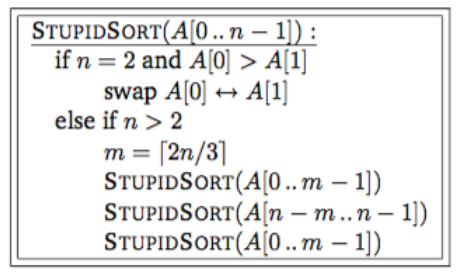
\includegraphics[width=0.4\textwidth]{./imagenes/stupidSort.png}
    \end{figure}

    \begin{enumerate}
        % Ejercicio 3.1
        \item Prove that \textsc{stupidsort} actually sorts its input.

        % Ejercicio 3.2
        \item Would the algorithm still sort correctly if we replaced 
        $m = \lceil \frac{2n}{3}\rceil$. Justify your answer.

        % Ejercicio 3.3
        \item Show that the number of swaps executed by \textsc{stupidsort} is
        at most $\big(\begin{smallmatrix} n \\ 2 \end{smallmatrix}\big)$.
    \end{enumerate}

    % Ejercicio 4.
    \item Supongamos que tenemos que ordenar una lista $L$ de $n$ enteros cuyos
    valores están entre $1$ y $m$. Pruebe que si $m$ es $O(n)$ entonces los 
    elementos de $L$ pueden ser ordenados en tiempo lineal. ¿Qué pasa si $m$ es 
    de $O(n^2)$? ¿Se puede realizar en tiempo lineal? ¿Por qué?

    % Ejercicio 5.
    \item Describe an algorithm that, given $n$ integers in the range $0$ to 
    $k$, preprocesses its input and then answers any query about how many of 
    the $n$ integers fall into a range $[a ... b]$ in $O(1)$ time. Your 
    algorithm should use $\Theta(n + k)$ preprocessing time.

    \textsc{Solución:}

    % Ejercicio 6.
    \item Sea $A$ un arreglo de $n$ elementos, tal que cada elemento se 
    encuentra a lo más a $k$ posiciones de su posición ordenada. Diseñe un 
    algoritmo que ordene $A$ en $O(n \log k)$.

    % Ejercicio 7.
    \item An abs-sorted array is an array of numbers in which $|A[i] \leq A[j|$
    whenever $i < j$. For example, the array $A = [-49, 75, 103, -147, 164, -197,
    -238, 314, 348, -422]$, though not sorted in the standard sence, is 
    abs-sorted. Design and algorithm that takes an abs-sorted array $A$ and a 
    number $k$, and returns a pair of indices of elements in $A$ that sum up to 
    $k$. For example, if $k = 167$ your algorithm should output $(3, 7)$. Output 
    $(-1, -1)$ if the is no such pair.

    % Ejercicio 8.
    \item \textbf{The Hogwarts Sorting Hat}

    Every year, upon their arrival at Hogwarts School of Witchcraft and Wizardry, 
    new students are sorted into one of four houses (Gryffindor, Hufflepuff, 
    Ravenclaw, or Slytherin) by the Hogwarts Sorting Hat. The student puts the 
    Hat on their head, and the Hat tells the student which house they will join. 
    This year, a failed experiment by Fred and George Weasley filled almost all 
    of Hogwarts with sticky brown goo, mere moments before the annual Sorting. 
    As a result, the Sorting had to take place in the basement hallways, where 
    there was so little room to move that the students had to stand in a long 
    line. After everyone learned what house they were in, the students tried to 
    group together by house, but there was too little room in the hallway for 
    more than one student to move at a time. Fortunately, the Sorting Hat took 
    Algorithms many years ago, so it knew how to group the students as quickly 
    as possible. What method did the Sorting Hat use? More formally, you are 
    given an array of n items, where each item has one of four possible values, 
    possibly with a pointer to some additional data. Design and analyze an 
    algorithm that rearranges the items into four clusters in $O(n)$ time 
    using only $O(1)$ extra space.

    \newpage
    % Ejercicio 8.
    \item Pruebe que el segundo elemento más chico de una lista de $n$ elementos 
    distintos puede encontrarse con $n + \lceil \log n \rceil - 2$ comparaciones.

    \begin{proof}
        Sea $T$ el árbol binario, en particular un \textit{min-Heap}, que 
        contiene a los $n$ elementos de nuestra lista en sus hojas. Por lo 
        discutido en clase, sabemos que para encontrar al elemento más pequeño 
        necesitamos realizar $n-1$ comparaciones, ya que al ir comparando los 
        elementos desde las hojas, vamos formando nuestros nodos internos (éstos 
        serán los elementos más pequeños de las comparaciones que se vayan 
        haciendo), los cuales siempre son $n-1$.

        Ahora bien, para encontrar al segundo elemento más pequeño debemos
        tener en cuenta una observación importante: como siempre vamos 
        \textit{subiendo} a los elementos más pequeños, eso quiere decir que el 
        segundo elemento más pequeño ya fue comparado con la raíz del árbol $T$,
        así que sólo queda ubicar a todos los elementos que \textit{perdieron}
        contra la raíz de $T$ y compararlos entre sí. Al ubicar estos elementos, 
        obtendremos que hay uno de ellos (a lo más) en cada nivel del árbol, y 
        como la altura del árbol es $\log_2 n$ entonces hacer esta última 
        pasada al árbol nos tomará $\lceil \log_2 n \rceil - 1$ comparaciones.
        Por lo tanto, encontrar al segundo elemento más pequeño de una lista de 
        $n$ elementos distintos nos toma 
        \begin{equation*}
            (n - 1) + (\lceil \log_2 n \rceil - 1) = n + \lceil \log_2 \rceil - 2
        \end{equation*}

        comparaciones.

        \begin{figure}[ht]
        \centering
        \forestset{default preamble={for tree={circle,draw}}}
        \begin{forest}
        [-1, red
          [-1,
            [-1
              [24, blue]
              [-1]
            ]
            [2, blue
              [2]
              [7]
            ]
          ]
          [0, blue
            [9]
            [0]
          ]
        ]
        \end{forest}
            
        \caption{Ejemplo de la explicación con la lista $[24, -1, 2, 7, 9, 0]$.
                 Los elementos en azul son aquellos que \textit{perdieron} contra 
                 el elemento más pequeño.}
        \end{figure}
    \end{proof}

\end{enumerate}
\end{document}
